    %===============================================================================
% LaTeX sjabloon voor de bachelorproef toegepaste informatica aan HOGENT
% Meer info op https://github.com/HoGentTIN/bachproef-latex-sjabloon
%===============================================================================

\documentclass{bachproef-tin}

\usepackage{hogent-thesis-titlepage} % Titelpagina conform aan HOGENT huisstijl
%\usepackage{graphicx}​​
\usepackage{array}
%%---------- Documenteigenschappen ---------------------------------------------

% De titel van het rapport/bachelorproef
\title{Docker of alternatieven als introductie tot container virtualisatie}

% Je eigen naam
\author{Eckhart Arents}

% De naam van je promotor (lector van de opleiding)
\promotor{Bert Van Vreckem}

% De naam van je co-promotor. Als je promotor ook je opdrachtgever is en je
% dus ook inhoudelijk begeleidt (en enkel dan!), mag je dit leeg laten.
\copromotor{Bert Van Vreckem}

% Indien je bachelorproef in opdracht van/in samenwerking met een bedrijf of
% externe organisatie geschreven is, geef je hier de naam. Zoniet laat je dit
% zoals het is.
\instelling{---}

% Academiejaar
\academiejaar{2020-2021}

% Examenperiode
%  - 1e semester = 1e examenperiode => 1
%  - 2e semester = 2e examenperiode => 2
%  - tweede zit  = 3e examenperiode => 3
\examenperiode{2}

%===============================================================================
% Inhoud document
%===============================================================================

\begin{document}

%---------- Taalselectie -------------------------------------------------------
% Als je je bachelorproef in het Engels schrijft, haal dan onderstaande regel
% uit commentaar. Let op: de tekst op de voorkaft blijft in het Nederlands, en
% dat is ook de bedoeling!

%\selectlanguage{english}

%---------- Titelblad ----------------------------------------------------------
\inserttitlepage

%---------- Samenvatting, voorwoord --------------------------------------------
\usechapterimagefalse
%%=============================================================================
%% Voorwoord
%%=============================================================================

\chapter*{\IfLanguageName{dutch}{Woord vooraf}{Preface}}
\label{ch:voorwoord}

%% :
%% Het voorwoord is het enige deel van de bachelorproef waar je vanuit je
%% eigen standpunt (``ik-vorm'') mag schrijven. Je kan hier bv. motiveren
%% waarom jij het onderwerp wil bespreken.
%% Vergeet ook niet te bedanken wie je geholpen/gesteund/... heeft

Toen bleek dat er vanuit de Hogeschool Gent interesse was in een onderzoek naar het gebruik van Docker of een gelijkaardige technologie om studenten met container virtualisatie te leren werken, was dit een uitdaging die mij sterk aansprak. Ik had hier en daar al gehoord van Docker en zelfs van Kubernetes, maar dit werd inderdaad nog niet behandeld aan de Hogeschool. Ik heb mij dan ook met veel plezier verdiept in de vernuftige wereld van container virtualisatie. Ik heb veel bijgeleerd over deze technologie en een eerste nuttige ervaring opgedaan in het gepast gebruik hiervan. Ik hoop dan ook dat de resultaten van mijn onderzoek er kunnen toe bijdragen dat in de toekomst andere studenten van de Hogeschool vlot zullen kunnen leren werken met deze technologieën. 

De persoon die ik het meest wens te bedanken voor zijn ondersteuning tijdens deze bachelorproef is ongetwijfeld Bert Van Vreckem. Hij was de lector vanuit de Hogeschool die het onderwerp naar voor bracht en daarmee ook mijn promotor. Onze opvolgingsgesprekken tussendoor mochten dan wel allemaal vanop afstand gebeuren, toch hebben ze mij iedere keer heel goed geholpen. Ze zorgden er voor dat ik de juiste focus hield en spoorden me telkens aan om met vernieuwde energie verder te doen. Tenslotte wens ik uiteraard ook mijn familie te danken. Mijn vader voor het nalezen van mijn teksten en mijn jongere zus voor het rekening houden met mijn werkplanning. Ze komt in haar eigen opleiding regelmatig problemen tegen met programmeren en heeft telkens wanneer ze mij om hulp wou vragen gewacht totdat mijn geplande tijd voor mijn onderzoeksactiviteiten gedaan was.
%%=============================================================================
%% Samenvatting
%%=============================================================================

% TODO: De "abstract" of samenvatting is een kernachtige (~ 1 blz. voor een
% thesis) synthese van het document.
%
% Deze aspecten moeten zeker aan bod komen:
% - Context: waarom is dit werk belangrijk?
% - Nood: waarom moest dit onderzocht worden?
% - Taak: wat heb je precies gedaan?
% - Object: wat staat in dit document geschreven?
% - Resultaat: wat was het resultaat?
% - Conclusie: wat is/zijn de belangrijkste conclusie(s)?
% - Perspectief: blijven er nog vragen open die in de toekomst nog kunnen
%    onderzocht worden? Wat is een mogelijk vervolg voor jouw onderzoek?
%
% LET OP! Een samenvatting is GEEN voorwoord!

%%---------- Nederlandse samenvatting -----------------------------------------
%
% TODO: Als je je bachelorproef in het Engels schrijft, moet je eerst een
% Nederlandse samenvatting invoegen. Haal daarvoor onderstaande code uit
% commentaar.
% Wie zijn bachelorproef in het Nederlands schrijft, kan dit negeren, de inhoud
% wordt niet in het document ingevoegd.

\IfLanguageName{english}{%
\selectlanguage{dutch}
\chapter*{Samenvatting}
\lipsum[1-4]
\selectlanguage{english}
}{}

%%---------- Samenvatting -----------------------------------------------------
% De samenvatting in de hoofdtaal van het document

\chapter*{\IfLanguageName{dutch}{Samenvatting}{Abstract}}

\lipsum[1-4]


%---------- Inhoudstafel -------------------------------------------------------
\pagestyle{empty} % Geen hoofding
\tableofcontents  % Voeg de inhoudstafel toe
\cleardoublepage  % Zorg dat volgende hoofstuk op een oneven pagina begint
\pagestyle{fancy} % Zet hoofding opnieuw aan

%---------- Lijst figuren, afkortingen, ... ------------------------------------

% Indien gewenst kan je hier een lijst van figuren/tabellen opgeven. Geef in
% dat geval je figuren/tabellen altijd een korte beschrijving:
%
%  \caption[korte beschrijving]{uitgebreide beschrijving}
%
% De korte beschrijving wordt gebruikt voor deze lijst, de uitgebreide staat bij
% de figuur of tabel zelf.

\listoffigures
\listoftables

% Als je een lijst van afkortingen of termen wil toevoegen, dan hoort die
% hier thuis. Gebruik bijvoorbeeld de ``glossaries'' package.
% https://www.overleaf.com/learn/latex/Glossaries

%---------- Kern ---------------------------------------------------------------

% De eerste hoofdstukken van een bachelorproef zijn meestal een inleiding op
% het onderwerp, literatuurstudie en verantwoording methodologie.
% Aarzel niet om een meer beschrijvende titel aan deze hoofstukken te geven of
% om bijvoorbeeld de inleiding en/of stand van zaken over meerdere hoofdstukken
% te verspreiden!

%%=============================================================================
%% Inleiding
%%=============================================================================

\chapter{\IfLanguageName{dutch}{Inleiding}{Introduction}}
\label{ch:inleiding}

Er is altijd al een nood geweest om software te kunnen draaien volledig onafhankelijk van de hardware en het besturingen systeem van een machine. De methodiek va een volledige virtual machine bestaat dan ook al een tijd. Een virtuele omgeving voorzie je het besturingssysteem van de hardware die wenst dat het heeft. Een probleem dat hier bij opkomt is dat het volledig besturing systeem niet altijd nodig is om een applicatie te draaien.  Zeek als je in een virtueel een omgeving maar één specifieke applicatie wilt draaien is de overhead van een besturingssysteem iets dat je kan missen.  Om één applicatie te draaien in een virtueel omgeving die het enkel voorziet van wat het nodig heeft is container virtualisatie in het leven geroepen. 
Het idee om in virtuele context een applicatie enkel toegang te geven tot wat het nodig heeft bestaat al lang, maar de recente populariteit van de container virtualisatie is voornamelijk te danken aan docker.  Docker slaagde erin het beheren en draaien van containers veel toegankelijker te maken dat de oudere manier waarmee Linux al werkte.  Verder heeft docker ook veel bijgedragen tot een standaard voor containers, hoe ziet een container er uit en hoe gedraagt het zich.  Deze standaard manier va het werken met containers en hun verticaliteit hielp ook bij het opzetten van de Cloud. Een container zal zicht het zelfde gedragen op elke server onafhankelijk van de onderliggende hardware. Bijkomend kunnen containers vlug bijgemaakt worden, zodanig dat als er een toename aan vraag is of er ergen een applicatie faalt het probleem snel opgelost geraakt. Idereen die met het technische deel van de Cloud in aanraking komt zou dus best kennis hebben van containers en hoe met deze te werken.


\section{\IfLanguageName{dutch}{Probleemstelling}{Problem Statement}}
\label{sec:probleemstelling}

Binnen de opleiding toegepaste informatica word de klassieke virtueel machine al aan bod gebracht, maar de Cloud en verwante technologieën kommen nog maar beperkt voor. Container virtualisatie is ook  iets dat zeer belangrijk is om mee te kunnen werken in een wereld waarbij je niet noodzakelijk de servers die je gebruikt fysiek bij jou hebt staan. De studenten kunnen voorbereiden op containers is dan ook meerwaarde voor de opleiding. 

\section{\IfLanguageName{dutch}{Onderzoeksvraag}{Research question}}
\label{sec:onderzoeksvraag}

Concreet is de vraag van deze thesis of dat Docker voldoet om als inleiding tot het gebruik van containers of dat een andere aanbieder beter zou zijn. Een aanbieder die net zoals docker iemand in staat stelt om lokaal op hun computer met containers te werken of een aanbieder die alles onmiddellijk  in de Cloud doet.
% Wees zo concreet mogelijk bij het formuleren van je onderzoeksvraag. Een onderzoeksvraag is trouwens iets waar nog niemand op dit moment een antwoord heeft (voor zover je kan nagaan). Het opzoeken van bestaande informatie (bv. ``welke tools bestaan er voor deze toepassing?'') is dus geen onderzoeksvraag. Je kan de onderzoeksvraag verder specifiëren in deelvragen. Bv.~als je onderzoek gaat over performantiemetingen, dan 

\section{\IfLanguageName{dutch}{Onderzoeksdoelstelling}{Research objective}}
\label{sec:onderzoeksdoelstelling}

Uit dit onderzoek moet duidelijk zijn dat Docker of een alternatief voldoet om gebruikt te worden als leermateriaal om met containers te werken. Dit door zowel een vergelijkende analyse van Dockers en zijn alternatieven, als het opzetten van een proof of concept demonstratie met de meest belovende technologieën.
Voor het aftoetsen van een mogelijk aanvaardbaar alternatief zijn er veel zaken die in het in rekening moeten worden gebracht worden, zeker voor het fungeren als les materiaal. Ten eerste moet het kunnen worden uitgevoerd worden op elk besturingssysteem. Ten tweede moet het uiteraard gebruiksvriendelijk genoeg zijn om op een redelijke hoeveelheid tijd besproken te worden.  Verder mag het studenten ook geen geld kosten. Lokaal moet het volledig gratis of een aanvaardbare trial periode doenbaar zijn. In een Cloud omgeving moet het doenbaar zijn binnen de perken van wat krediet op de Cloud service waarop de student recht zou hebben. Tenslote zou het effectief opzetten van de Drupal site met de technologie, gebruik makende van containers, niet langer dan 4 uur mogen duren.
% Wat is het beoogde resultaat van je bachelorproef? Wat zijn de criteria voor succes? Beschrijf die zo concreet mogelijk. Gaat het bv. om een proof-of-concept, een prototype, een verslag met aanbevelingen, een vergelijkende studie, enz.

\section{\IfLanguageName{dutch}{Opzet van deze bachelorproef}{Structure of this bachelor thesis}}
\label{sec:opzet-bachelorproef}

% Het is gebruikelijk aan het einde van de inleiding een overzicht te
% geven van de opbouw van de rest van de tekst. Deze sectie bevat al een aanzet
% die je kan aanvullen/aanpassen in functie van je eigen tekst.

De rest van deze bachelorproef is als volgt opgebouwd:

In Hoofdstuk~\ref{ch:stand-van-zaken} wordt een overzicht gegeven van de stand van zaken binnen het onderzoeksdomein, op basis van een literatuurstudie.

In Hoofdstuk~\ref{ch:methodologie} wordt de methodologie toegelicht en worden de gebruikte onderzoekstechnieken besproken om een antwoord te kunnen formuleren op de onderzoeksvragen.

% TODO: Vul hier aan voor je eigen hoofstukken, één of twee zinnen per hoofdstuk

In Hoofdstuk~\ref{ch:conclusie}, tenslotte, wordt de conclusie gegeven en een antwoord geformuleerd op de onderzoeksvragen. Daarbij wordt ook een aanzet gegeven voor toekomstig onderzoek binnen dit domein.
\chapter{\IfLanguageName{dutch}{Stand van zaken}{State of the art}}
\label{ch:stand-van-zaken}
Dit deel begint met een inleiding over virtualisatie, de reden om virtualisatie te doen en de verschillende soorten. Daarna worden Virtuele machines en Hypervisors besproken. Gevolgd door een geschiedenis en ontstaan van container virtualisatie en de  effectieve werking van ervan. Om vervolgens een vergelijking tussen Virtuele machines en Container virtualisatie te schetsen. Dit deel wordt afgesloten met het overlopen van een aantal aanbieders van software voor container virtualisatie. 

% Tip: Begin elk hoofdstuk met een paragraaf inleiding die beschrijft hoe
% dit hoofdstuk past binnen het geheel van de bachelorproef. Geef in het
% bijzonder aan wat de link is met het vorige en volgende hoofdstuk.

% Pas na deze inleidende paragraaf komt de eerste sectiehoofding.
\section{Wat is virtualisatie}

Virtualisatie is in essentie het maken van een abstractie van de onderliggende hardware waarop  software berust tijdens het uitvoeren van processen. Naast de hardware laat virtualisatie ook toe om het besturingssysteem waarmee de software de hardware aanspreekt naar de hand te zetten. Een eerste reden om aan virtualisatie te doen is om mogelijke verschillen in hardware en besturingssystemen uit te sluiten.  Software dat ontwikkeld wordt in een omgeving met zekere hardware en besturingssysteem kan zich anders gedragen of zelfs incompatibel zijn met de omgeving waarin de software effectief in productie gebruikt  moet worden. Een verder voordeel dat virtualisatie toelaat is een betere benutting van hardware, zeker bij servers. De fysieke hardware van een server kan door middel van virtualisatie  gebruikt worden om meerdere applicaties draaien die elk andere vereisten hebben. Ook hier help de abstractie van de oorspronkelijke hardware en eventuele besturingssysteem van de server een gebruiker die software wilt draaien op een server om dit te kunnen zonder de hardware van de server te moeten kennen \Autocite{Yadav2018,Jangla2018}.

Voor virtualisatie bestaan er verschillende manieren van aanpak. Een eerste is de virtuele machine manier wat in volgend deel besproken wordt. En tweede manier is van gedachte om de virtualisatie van software te kunnen beheren  op analoge wijze als Vrachtcontainers. Ten derde is er ook nog emulatie, een vorm van virtualisatie die niet verder behandeld wordt in deze thesis.

\section{Virtuele machines en Hypervisors}

\subsection{Virtuele machines}
Een eerste manier van virtualisatie is een volledige virtuele machine (VM). Bij VM wordt er virtuele hardware voorzien van een eigen besturingssysteem. Aan de hand van dit besturingssysteem en de virtuele hardware is het dan ook mogelijk om in deze VM een applicatie te draaien alsof hij op een echte machine staat. Verder zorgt deze virtualisatie ervoor dat het draaien van een applicatie in een VM volledig hetzelfde zal blijven zou de VM zelf op andere hardware berusten. Het besturingssysteem dat in de VM draait is volledig configureerbaar waardoor het mogelijk is om andere soorten toestellen te nabootsen, zoals een gsm. Een VM zelf is niets meer dan de ruimte op de opslag schijf die het gebruikt voor zijn eigen instellingen en zijn eigen interne bestanden te bewaren. Wegens de aanwezigheid van een volledige besturingssysteem kan de geheugenruimte die een VM inneemt groot. Het direct aanspreken van bestanden in het interne geheugen van een VM laagst buitenaf zonder via de VM’s kanalen te werken is ook standaard niet mogelijk\autocite{Eder2016}.

\subsection{Hypervisor}

Omdat een VM beschouwd kan worden als gewoon een deel van het geheugen dat gebruikt wordt om het op te slaan is er nood aan bijkomende software om de VM effectief bruikbaar te maken. Deze bijkomende software wordt een Hypervisor genoemd. De Hypervisor staat voornamelijk in voor het vertalen van input die de VM naar zijn eigen virtuele hardware stuurt te vertalen en om te zetten zodat ze door de werkelijke hardware uitgevoerd kunnen worden. De virtuele kernel van de VM dus dankzij de hypervisor effectief uitgevoerd. Een Hypervisor blijft niet bij het beheren van maar één VM, het laat ook toe om nieuwe VM’s aan te maken door middel van het alloceren van geheugenruimte en de virtuele hardware voor te bereiden om een besturingssysteem op te zetten. Aansluiten laat de Hypervisor dan ook toe dat er meerdere VM’s tegelijkertijd in gebruik kunnen worden genomen.  Vaak laat een hypervisor ook toe om op een eenvoudige manier de VM van buitenaf te bereiken. Hetzij via een bestand locatie te organiseren die je zowel via de VM als van buiten af kunt bereiken of het klaarzetten van virtuele netwerken waarmee de VM’s onderling of naar buiten kunnen communiceren.

Onder Hypervisors zijn er twee verschillende  types te onderscheiden. Type 1 Hypervisors staan zelf direct op de hardware van de machine. Hierdoor heeft de hardware geen directe besturingssysteem, en spreekt de hypervisor direct de machine kernel aan voor de uitvoering van opdrachten. De  een zijn de besturingssystemen die aanwezig zijn enkel deze die als gast door de Hypervisor in een VM worden uitgevoerd op de hardware. Type 2 Hypervisors daarentegen worden uitgevoerd als een gebruikers applicatie binnen een host besturingssysteem.  De VM’s draaien genest in een conventioneel besturingssysteem en omgeving die gebruikt kan worden. een verschil tussen de twee wordt geïllustreerd in figuur 1 \autocite{Yadav2018,Eder2016}.

%TODO: figuur 1 maken


\section{Container virtualisatie}

Bij container virtualisatie is de kerngedachte om enkel te virtualiseren wat de applicatie die effectief nodig heeft. De applicatie zelf en alle dependencies die het nodig heeft worden gebundeld in een ‘container’ die overal kan worden gebruikt. In deze vorm van virtualisatie wordt de hardware en besturingssysteem niet gevirtualiseerd, de containers spreken zelf het besturingssysteem van de host aan om procestijd en andere hardware middelen aan te spreken. Doordat het beeld, ook image genoemd, van een container minder bijhoud dan dat van een VM zijn ze kleiner en starten ze sneller op \autocite{Eder2016,jangla2018}.

\subsection{korte geschiedenis van container virtualisatie}

Een oudere manier van container virtualisatie bestaat al lang in de vorm van de \textbf{ch}ange \textbf{root} functionaliteit in unix gebaseerde besturingssystemen. Met Chroot is het sinds 1982 mogelijk om de root directory van proces, en zijn sub processen, aan te passen en zo te limiter waartoe het proces toegang heeft. Vanuit chroot is het Linux containers (LXC) project\footnote{\url{https://linuxcontainers.org/}} gestart en werd het in 2008 mogelijk om Linux gebaseerde container virtualisatie te doen via de ontwikkelde toolkit. Met deze toolkit is het iets eenvoudiger om containers te maken maar is er nog veel kennis van de Linux kernel nodig\autocite{Eder2016,SenthilKumaran2017}.

In 2013 kwam Docker\footnote{\url{https://www.docker.com/}} op de markt en slaagde erin om het werken met Linux gebaseerde container veel te vereenvoudigen ten opzichte van LXC’s toolkit. Door Docker’s succes in het vereenvoudigen van de workflow voor het creëren en draaien van containers is de technologie dan ook in een versnelling terecht gekomen.  Een grote vernieuwingen die Docker zelf bracht was het werken met duidelijke container images voor het maken en bewaren van containers. Hierbij bied het ook de Docker hub aan om deze images te bewaren en te delen. Dockers succes werd verder ondersteunt doordat google  al zelf een tijd intern zelf werkte en zo geschikte software kon aanbieden om gebruiksvriendelijk  meerdere containers tegelijkertijd te beheren. In 2016 publiceerde google een retrospectieve die uitgelegde hoe het al een aantal jaren met Linux gebaseerde containers werkte door middel van oudere software Borg en Omega, en hiermee Kubernetes{\url{https://kubernetes.io/}} ontwikkelde. De gebruiksvriendelijkheid en voordelen die de lichter virtualisatie kan bieden zorgden er dan ook voor dat container virtualisatie door velen werd geadopteerd \autocite{Eder2016}.

\subsection{Engine}

Voor het aanmaken en draaien van containers op een systeem is er nood aan een container manager of engine. Met een container engine is het mogelijk om een container image te draaien of aan de hand van een image meerdere containers van dezelfde applicatie te maken. Het effectief draaien van de container wordt gedaan aan de hand van een runtime dat vaak gebundeld zit in de engine de rest van de functionaliteiten is eigen aan de engine. De levenscyclus van een container te laten beheren door een engine begint met het ophalen van een container image om van te vertrekken. Deze kunnen gedownload worden van een publieke of privé repository van images. Dit vertrekpunt kan dan verder worden aangepast voor de specifieke applicatie noden vooraleer terug opgeslagen te worden in een repository. Hierna kan de image effectief gebouwd worden om te draaien als een container applicatie. Een container engine kan software zijn die on- premise geïnstalleerd is, waardoor de configuratie zelf te doen is, of het kan worden aangeboden door een Cloud service provider, zodat er in deze Cloud omgeving zonder te veel configuratie met containers kan worden gewerkt\autocite{Casalicchio2020}.

\subsection{Orchestration}
Om grotere hoeveelheden diverse container applicaties te kunnen beheren is er Container Orchestration (CO) software. CO is vooral gericht naar het beheren van Multi-level applicaties waar van de delen in containers draaien. Met CO kan er eenvoudiger geconfigureerd worden hoe verschillende container applicatie met elkaar moeten verbinden en is het zelf mogelijk om deze communicatie over meerdere fysieke servers te spreiden. Een andere functionaliteit die CO’s vaak hebben is het beheren van fouttolerantie en het opschalen van aanbod. Hiermee kan er bij toenemende nood aan container applicaties of  bij uitval van een container, extra containers aangemaakt worden en opgenomen worden in het systeem. Ook voor Orchestration is er een onderscheiding tussen on-premise software of CO als deel van het aanbod van een Cloud service provider met container ondersteuning\autocite{Casalicchio2020,Truyen2019}.

%TODO: een figuur voor container virtualisatie

\section{Verschillen tussen virtuele machines en containers}
%TODO: zij bij zij vergelijking van contaier en VM + figuur

\subsection{Performantie verschillen}
Een vergelijkende studie tussen Containers en virtuele machine gebaseerde virtualisatie\autocite{Yadav2018} haalt aan dat de verschillende manieren van virtualisatie elk hun voordelen en nadelen hebben en dat het afhangt van de noden van de huidige situatie. Dit onderzoek haalt enkel voordelen aan die containers hebben ten opzichte van VM’s zoals: minder nood aan geheugen ruimte, snellere boot-up en hogere draagbaarheid van containers. Maar haalt ook aan de beveiliging bij containers moeilijker is doordat containers direct de host kernel en hardware aanspreken. In een Cloud omgeving zullen zowel VM’s als container virtualisatie hun plaats hebben. Zo zijn VM’s beter geschikt voor Interface as a Service Cloud solution of situaties waar beveiliging van zeer hoog belang is. Terwijl Containers meer toepasbaar is voor Software as a Service.

Een gelijkaardige studie door \textcite{Eder2016} komt tot gelijkaardige conclusies. VM’s en hypervisors zijn een extra laag beveiliging bij virtualisatie. Containers hebben het voordeel van sneller en eenvoudiger te zijn waardoor ze zeer toepasbaar zijn in de cloud omgeving.

Een onderzoek van \textcite{Abdullah2019} heeft vooral gezocht naar de verschillen in opschalen van Multi-level applicaties in een container of VM gebaseerd netwerk. Zij concludeerden dat container based virtualisatie beter is om toenemende vraag aan te kunnen.


\section{Software aanbieders}
In dit deel komen verschillende software pakketten en aanbieders van software voor container virtualisatie aan bod. Beginnende met software voor container engines en runtimes gevolgd door orchestrion.  Hierna de aanbieders van platformen voor het hosten en delen van container images. Ten slotte enkele grote Cloud service providers en hun ondersteuning van containers in hun Cloud omgeving.


\subsection{Open Container Initiative}
Om de onderlinge werking en overdraagbaarheid tussen alle mogelijke software te waarborgen is het Open container Initiative(OCI)\footnote{\url{https://opencontainers.org/}} tot stand gebracht. Om dit mogelijk te maken legt het twee standaarden voor. De eerste standaard is de runtime specificatie voor het draaien van containers. De tweede standaard is voor het bewaren van de image van een container.


\subsection{Engines en runtimes}

\paragraph{Docker engine}
De runtime en daemon waarmee Docker werkt heet de Docker engine. De daemon zelf is gebaseerd op Containers wat hierna besproken wordt. Het werkt via een Command-line-interface (CLI) om zolang dat de daemon draait containers te kunnen starten, aanmaken of verwijderen. Het laat ook toe huidige containers aan te spreken en status op te halen. De Docker engine word voor Mac os en Windows gebundeld met de Docker desktop, een user interface om de werking van de engine te beheren zonder via de CLI  te moeten werken. De Docker engine is dan ook bruikbaar op alle vaak voorkomende besturingssystemen, maar Linux distributies hebben momenteel geen toegang tot de Docker desktop.
\paragraph{Containered}
Containered\footnote{\url{https://containerd.io/}} is een industriestandaard runtime om op Linux en Windows systemen containers te draaien. Door Middel van Go programma’s kan Containered een container image pullen, configureren, opstarten en beëindigen.
linux containers
Zoals eerder aangehaald is Linux containers een manier om met containers te werken op Linux. Het vergt veel kennis van de Linux kernel om goed te kunnen gebruiken.  Het omslaat zowel de LXC manier om containers te maken en draaien. Als een uitbreiding van LXC onder de vorm van LXD. LXC is standaard toegevoegd als deel van veel van de Linux distributies.  
\paragraph{CRI-O}
Cri-o\footnote{\url{https://cri-o.io/}} is een engine die zichzelf verkoopt als een lichter alternatief voor de Docker engine.  Via Cri-o kan op een Linux besturingssysteem via de command line gewerkt worden om eender welk OCI compliant image en runtime te beheren via Kubernetes.
\paragraph{Podman}
Podman\footnote{\url{https://podman.io/}} is nog een andere CLI om OCI compliant containers te creëren, draaien en stoppen op een Linux systeem. Naast de command line heeft het ook een RESTful API en service om de containers aan te spreken. De API kan via de Podman remote client gebruikt worden om de engine extern te sturen. De remote client het ook versies voor Windows en Mac os om vanuit deze besturingssystemen Podman in zijn Linux omgeving te kunnen aanspreken.
\paragraph{Windows containers}
Windows Containers\footnote{\url{https://docs.microsoft.com/en-us/virtualization/windowscontainers/about/}} is een specifieke runtime om Windows gebaseerde containers uit te voeren. Het heeft geen eigen engine en berust op integratie met Docker engine en de Docker desktop voor de verdere functionaliteiten.  Het draaien van Windows containers is mogelijk op de Server en Enterprise edities van Windows.
\paragraph{Pouch containers}
Pouch containers\footnote{\url{https://pouchcontainer.io/}} is een open source engine voor Linux containers gestart door de Alibaba Group\footnote{\url{https://www.alibabagroup.com/en/global/home}}. het ondersteunt Linux als besturingssysteem en Werkt ook voornamelijk via command line. Het is ook OCI compliant. en heeft een laatste stabiele release in juni 2019.
\paragraph{Kata containers}
Kata containers\footnote{\url{https://katacontainers.io/}} combineert de beveiligingen voordelen van VM met de draagbaarheid van containers.  Het is een open source runtime en berust op een andere engine voor  de engine functionaliteiten zoals CRI-O en Containered. het kan gebruikt worden op vele Linux distributies en heeft ondersteuning in de vier Cloud omgevingen van de providers die later aan bod komen.
\paragraph{Andere engine opties}
Veel van de volgende opties voor engines zijn niet meer goed ondersteunt.
\begin{itemize}
    \item Open vz\footnote{\url{https://openvz.org/}}: Een open source benadering om in Linux zowel containers als virtuele machines te draaien, weinig activiteit sinds 2015.
    \item Rkt\footnote{\url{https://www.openshift.com/learn/topics/rkt}}: Een engine voor container linux containers dat na de RedHat acquisitie niet meer ondersteunt wordt  laatste release was 2018.
    \item Balena engine\footnote{\url{https://github.com/balena-os/balena-engine}}: een specifieke engine voor Internet of Things toepassingen.  Laatste release was December 2019.
    \item Flockport\footnote{\url{https://www.flockport.com/}}:open source engine met ook wat orchestrion functionaliteiten voor enkele van de meest voorkomende Linux distributies. De open source is niet terug te vinden en heeft bijna geen activiteit op de officiële website sinds 2019
\end{itemize}


\subsection{Orchestrion}
%TODO: Aanvullen OC
\paragraph{Docker compose en swarm}
\paragraph{Kubernetes}
\paragraph{Nomad}
\paragraph{Apache Mesos}
\paragraph{Openstack}
\paragraph{openshift}
\subsection{Image repositories}
Om container images te kunnen delen met andere zijn er repositories die deze remote kunnen bewaren, Om ze snel te kunnen kopiëren naar een lokale omgeving. Naast de drie die in dit deel besproken worden bieden Cloud providers ook hun eigen repositories aan voor intern binnen hun Cloud omgeving te gebruiken.
\paragraph{Docker hub}
De docker hub\footnote{\url{https://hub.docker.com/}} is de grootste en meest gekende Repository voor container images. het heeft zo een grote bibliotheek aan images. veel vaak gebruikte images worden dan ook gehost op de docker hub en docker help ook bij het erkennen van officiële images. Voor het hosten van eigen images op de Docker zijn publieke images gratis. Voor private images moet er betaald worden. publieke images kunnen ook anoniem opgehaald worden.
\paragraph{GitHub container registery}
Github werkt aan een functionaliteit om als gebruiker of onderneming op github container images te bewaren genaamd de  GitHub container registery\footnote{\url{https://docs.github.com/en/packages/guides/about-github-container-registry}}. Het ondersteund zowel Docker’s eigen images als De OCI images. Het is een deel van GitHub’s packages en is momenteel nog in Beta. De container registery wijkt af van de GitHub packages in mate dat de container images niet gekoppeld moeten zijn met een github repository. Hierdoor zijn de toegangsrechten van de images onafhankelijk van eventuele repositories waartoe ze behoren en kunnen deze afzonderlijk ingesteld worden. Bijkomend is het mogelijk om een publiek gedeelde container image anoniem te downloaden wat met gewone packages niet toegestaan is. Tijdens De Beta is het gebruik van de container registery volledig gratis. Eens het uit beta is zal de Container registery samen met de rest van de GitHub packages gefactureerd woorden. Namelijk publieke bestanden gratis, en een limiet op bestands grootte en data overdracht voor private images.
\paragraph{Gitlab container registery}
%TODO:  aanvullen gitlab


\subsection{Cloud hosting en services}
%TODO: aanvullen cloud
\paragraph{Amazon AWS}
\paragraph{Microsoft Azure}
\paragraph{Google cloud}
\paragraph{Red Hat OpenStack Platform}




%%=============================================================================
%% Methodologie
%%=============================================================================

\chapter{\IfLanguageName{dutch}{Methodologie}{Methodology}}
\label{ch:methodologie}
In dit deel wordt eerst overlopen aan welke voorwaarden software moet voldoen om te kunnen dienen als leermiddel. Vervolgens worden deze voorwaarden afgetoetst aan de gevonden software om zoo een aantal test omgevingen voor te definiëren. Hierna woorden de resultaten van de tests besproken om af te sluiten met algemeen resultaat.

%% Hoe ben je te werk gegaan? Verdeel je onderzoek in grote fasen, en
%% licht in elke fase toe welke stappen je gevolgd hebt. Verantwoord waarom je
%% op deze manier te werk gegaan bent. Je moet kunnen aantonen dat je de best
%% mogelijke manier toegepast hebt om een antwoord te vinden op de
%% onderzoeksvraag.

\section{Selectie software}
Om software te vinden die toepasbaar is om gebruikt te worden als lesmateriaal moeten er bepaalde vereisten voldaan zijn.

\begin{itemize}
    \item Kosteloos zijn; als er kosten zijn mogen deze de leer ervaring niet ten nadele komen.
    \item Uitvoerbaar op de computers van de studenten. Mag door de verschillen in besturingssystemen van studenten computers niet te veel verschillen in werking.
    \item De software moet op zichzelf of in combinatie met ander software de volledige levenscyclus van containers kunnen tonen en niet te restrictief in gebruik zijn.
    \item Niet te complex zijn om te gebruiken.
    \item Geen verwaarloosde software zijn.
\end{itemize}
    
\subsection{Algemene toepassing voorwaarden op gevonden software}
Door een klassieke VM te gebruiken om daarin te werken kunnen de problemen met de uitvoerbaarheid op het gast besturingssystemen vermeden worden en zal de ingebruikname ook binnen de VM voor alle studenten hetzelfde zijn. Dit heeft ook het voordeel dat het besturingssysteem van de VM een Linux distributie kan zijn, een voorwaarde die nodig is om veel van software te kunnen draaien. De rest van deze sectie zal iets specifieker de gevonden technologieën overlopen.

Met uitzondering van technologieën die op Cloud berusten, de repositories of volledige Cloud services, zijn alle van de gevonden technologieën gratis te gebruiken. Ook is er door het OCI een zekere mate van mudulariteit tussen de technologieën. Software mag dan zelf niet de volledige orchestration kunnen doen, zal er een zekere integratie zijn met software dit dat wel kan.

\subsection{Engines en runtimes}
Qua geschiktheid om als runtime komen Docker engine en Podman het beste uit. Docker Dankzij zijn populariteit en veelvuldigheid. Hiermee is er ook veel onlinehulp te vinden voor het gebruik van Docker. Podman ’s vriendelijkheid als leermiddel is deels te danken doordat het zich opstelt als een duidelijk alternatief voor Docker op Linux distributies. De directe hulp een uitleg om met Podman te werken mag dan al iets minder zijn, die werking van Podman zou kort beschreven kunnen worden als hetzelfde als dat van Docker qua commando’s met een ingebouwde ondersteuning voor pods van meerdere containers.  Verder zou Containerd ook nog een alternatief kunnen zijn maar dan nipt op de rand van de complexiteit, zeker in vergelijking met Podman en Docker.

Om zelf te werken met Linux containers is te complex om een goede introductie tot containers te zijn. Windows containers zijn enkel mogelijk op bepaalde distributie van Windows en berusten verder op de Docker engine voor de uitvoering, hierdoor is de extra stap om met deze containers te werken ten opzichte van Docker geen meerwaarde als inleiding. Een gebrek aan uitleg voor het gebruik van cri-o doet twijfelen aan de geschiktheid voor Cri-o als runtime.  Het unieke verkooppunt van Kata containers, de mogelijkheid om ook VM’s als containers te draaien is een stap in complexiteit te ver om een goede inleiding to container virtualisatie te zijn.  De rest van de gevonden runtimes zijn te klein of al te lang zonder ondersteuning om met zekerheid te kunnen zeggen dat ze relevant zullen blijven voor containers en verwante technologieën.

\subsection{Orchestration}
Docker compose is een uitbreiding van de Docker engine en is daarmee ook gratis en heeft dezelfde vereisten als Docker, het wordt zelf standaard geïnstalleerd met de Docker desktop applicatie. Kubernetes en Nomad zijn verder nog twee softwarepakketten die goed zouden kunnen zijn om met te leren. Kubernetes is de meest gebruikte orchestration software en is daarmee zoals Docker voorzien van veel online tutorial. Het is open source en kan met veel van de runtimes werken. Voor het leren werken met Kubernetes is er ook Minikube die je lokaal in staat stel met Kubernetes te werken. Nomad is orchestration software die lijkt op Kubernetes maar toch zichzelf wilt onderscheiden van Kubernetes door meer dan alleen containers te kunnen beheren. 

De specifieke besturingen systemen orchestration DC/OS en Apache Mesos zijn te gelimiteerd tot het besturingssysteem en verder ook te complex om een duidelijke introductie te zijn tot container virtualisatie.  Openshift is een te commercieel en bedrijfsgericht product om makkelijk in gebruikt e worden genomen. En tenslotte is er nog de Docker swarm die zelf aan populariteit verliest ten opzichte van Kubernetes als software voor orchestration.


\subsection{Image repositories}
Met dat het OCI en hun container image geslaagd is in de standaardisatie container images zijn repositories vrij met elkaar te verwisselen. De Docker hub en de GitHub container registry zijn de meest geschikt om door een student als image repository te gebruiken.  Docker hub doordat het bijna overal als standaard gebruikt wordt en de GitHub omdat een student wellicht al een GitHub account hebben. Ook de kostenstructuur van de twee is te vergelijken met gratis publieke images en betaling vanaf een bepaalde drempel voor private images. Tijden het schrijven van deze thesis is de GitHub container registry wel no in een bètafase waardoor het volledig gebruik gratis is.

\subsection{Cloud hosting en servces}
Cloud hosting services kunnen een optie zijn maar afhankelijk van de host kan het dat een free trial niet toegang geeft tot alle tools die nodig zijn of is het moeilijk om gratis krediet te krijgen. Zo geeft Amazon geen gratis krediet meer of vraagt Google voor een creditcard.  Verder zal het maken van een image eerst lokaal moeten gebeuren waarvoor een lokale runtime nodig is. Hierdoor kan er even goed in eerste instantie lokaal verder gewerkt worden.

\section{Software Tests}
Wegens de modulariteit gecreëerd door het OCI zullen eerst de runtimes uitgeprobeerd worden om daarna te kijken naar de mogelijkheden van de runtimes om te werken met toegewijde orchestration software.

\subsection{Runtimes}
Voor deze is het voornaamste belang dat containers kunne gemaakt gedraaid en gestopt worden door middel van de runtime ook moet het persisteren van data naar een volume en het pullen van een image mogelijk zijn.

\paragraph{Docker Desktop}
De Docker desktop een applicatie voor Windows en Mac die Dockers engine combineert met Docker-compose, lokale Kubernetes, een dashboard en een eenvoudige verbinding met de Docker hub. Wegens de volledigheid van deze bundel zal dit als eerste uitgeprobeerd worden. Doordat de desktop applicatie niet voor Linux bestaat is deze echter niet volledig toepasbaar voor alle studenten. Een Linux gebruiker zou de delen apart moeten installeren. Dit is ook de software die direct op een laptop zal worden uitgevoerd en niet in een VM. Ook zal dit gebruikt worden als een baseline voor vergelijkingen. 

\paragraph{Fedora Podman}
Een eerste VM waarin het meest beloftevolle alternatief wordt getest is Fedora workstation instantie. Deels omdat Fedora al gebruikt wordt tijdens het vak besturingssystemen en omdat het ook standaard met een Firefox webbrowser komt waarmee het gemakkelijk is om te testen of een webservice gebaseerde container draait.

\paragraph{Ubuntu Podman}
Om Podman ook uit te proberen op een ander besturingssysteem dan Fedora zal ook eens geprobeerd worden of dat het lukt om Podman te installeren op een Ubuntu distributie.

\subsection{Orchestration}
Voor orchestration moet het mogelijk zijn om een job of taak op basis van containers te maken, aan te passen en te stoppen. En ook om iets complexer dan een enkele container service te draaien.

\paragraph{Kubernetes gebundeld met Docker desktop}
De Docker desktop applicatie komt met de mogelijkheid om een lokale Kubernetes instantie te starten. Het lijkt dus interessant om Deze ook eens te testen.

\paragraph{Podman met Minikube voor Kubernetes}
Om te testen of dat het ook mogelijk is om met Podman als runtime te werken voor Kubernetes zal er ook geprobeerd worden om een Minikube instantie werkende met Podman op te zetten en gebruiken.

\paragraph{Docker engine en Nomad}
In tegenstelling tot Kubernetes en Minikube die meer vrijheid heeft voor de achterliggende runtime heeft Nomad op dit moment enkel ondersteuning voor de Docker engine om mee te werken voor het draaien van een containers. Dus voor het uitproberen van Nomad moet er met een Docker engine gewerkt worden.

\section{Resultaten software Tests}
In dit deel worden de resultaten en ondervindingen van het werken met de eerder opgestelde software test scenario’s overlopen. 

\subsection{Docker Desktop}
Het eerste dat uitgeprobeerd werd is de Docker desktop geïnstalleerd als applicatie op een laptop met 8 GB ram geheugen.

\paragraph{Installatie en set-up}
Het werken met Docker desktop direct geïnstalleerd op een Windows systeem moet er eerst het Windows Subsysteem voor Linux ingeschakeld worden. Docker verwijst hiervoor naar de help pagina’s van Microsoft. Hiervoor werden de manuele instructies van Microsoft \footnote{\url{https://docs.microsoft.com/en-us/windows/wsl/install-win10}} gevolgd om tot en met het opzetten van WSL2 als default uit te voeren. Het enigste dat hier wat specifieke aandacht vereist ten opzichte van de beschreven stappen is het controleren of dat de Windows versie geschikt is voor WSL.

Hierna werd de installer van Docker desktop uitvoeren, dit heeft een optie om WSL voor de gebruiker voor te bereiden maar omdat dit reeds gedaan was is er niet kunnen getest worden of dat dit het volledig ennablen van WSL doet of enkel verantwoordelijk is voor het instellen van een Linux distributie in WSL waarmee de containers zullen worden uitgevoerd.

\paragraph{Ingebruikname}
Bij het eerste keer opstarten van de desktop applicatie staart het et een korte tutorial die enkel het pullen builden en uitvoeren van een eenvoudige container behandelt,  dit deels op een zeer korte introductie te zijn en te testen of dat de installatie gelukt is. Eveneens is het opstarten van de desktop applicatie de trigger om de backend die alles effectief draait ook te starten.

Vervolgens werd een uitgebreide tutorial van Docker gevolgd\footnote{\url{https://docs.docker.com/get-started/02_our_app/}}. Deze legde het werken met Docker en Docker compose zorgvuldig uit. Beginnende met een git repository die je zelf moet clonen om daarvan aan de hand van een Dockerfile, te zien in figuur \ref{fig:dockerfilevscode}, een image te bouwen. Vervolgens deze image eens lokaal draaien, updaten en pushen naar de Docker hub. De Docker desktop applicatie werd ook gehanteerd om te demonstreren dat je deze dashboard ook je containers kan starten stoppen, pushen of verwijderen. een voorbeeld van hoe de desktop applicatie eruit ziet is in figuur \ref{fig:Dockerdesktop} te zien. De gepushte image kon vervolgens op een Play with Docker omgeving eens worden uitgevoerd om de overdraagbaarheid te demonstreren. Het werken met volumes voor het persisteren van data werd ook behandelt. 

\begin{figure}[h]
    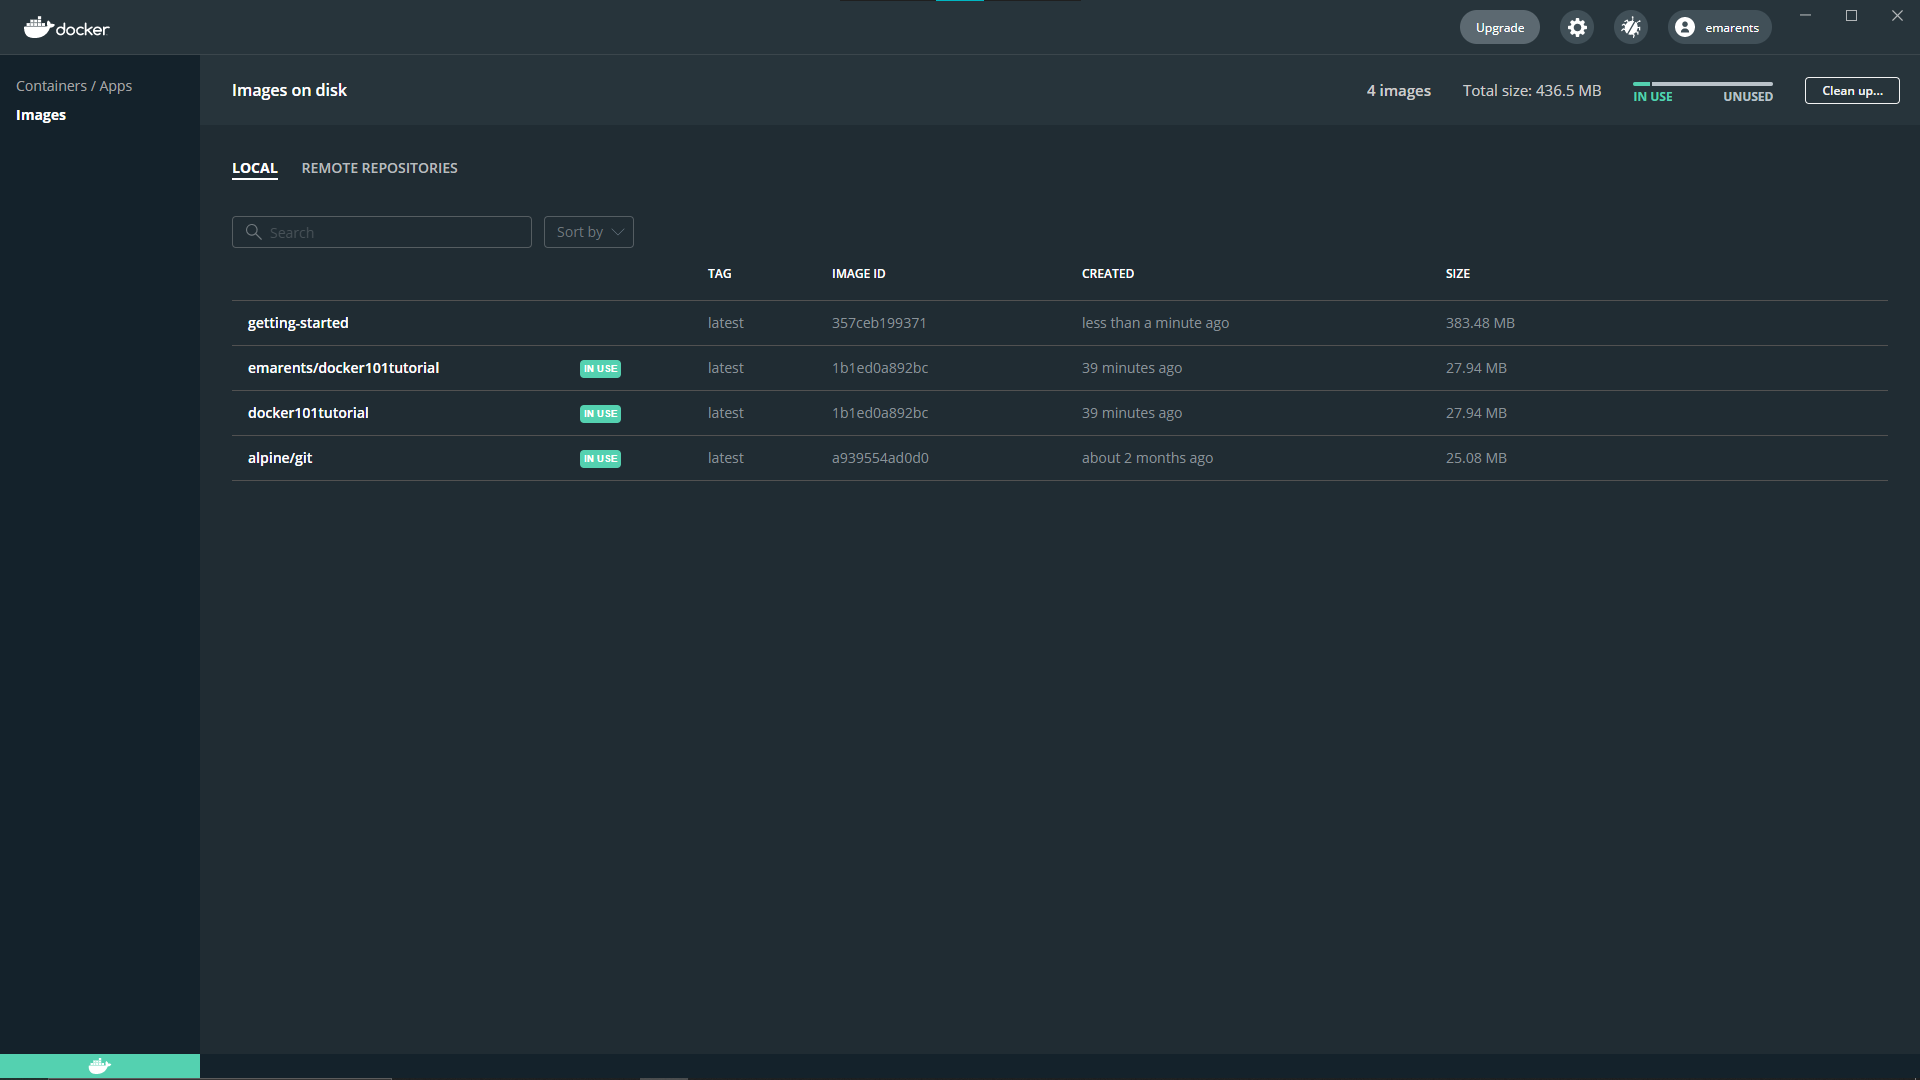
\includegraphics[width=\linewidth]{img/dockerImg.png}
    \label{fig:Dockerdesktop}
    \caption[De Docker desktop applicatie]{De Docker desktop applicatie, dit deel toont alle lokaal bewaarde images}
    \centering
\end{figure}
\begin{figure}[h]
    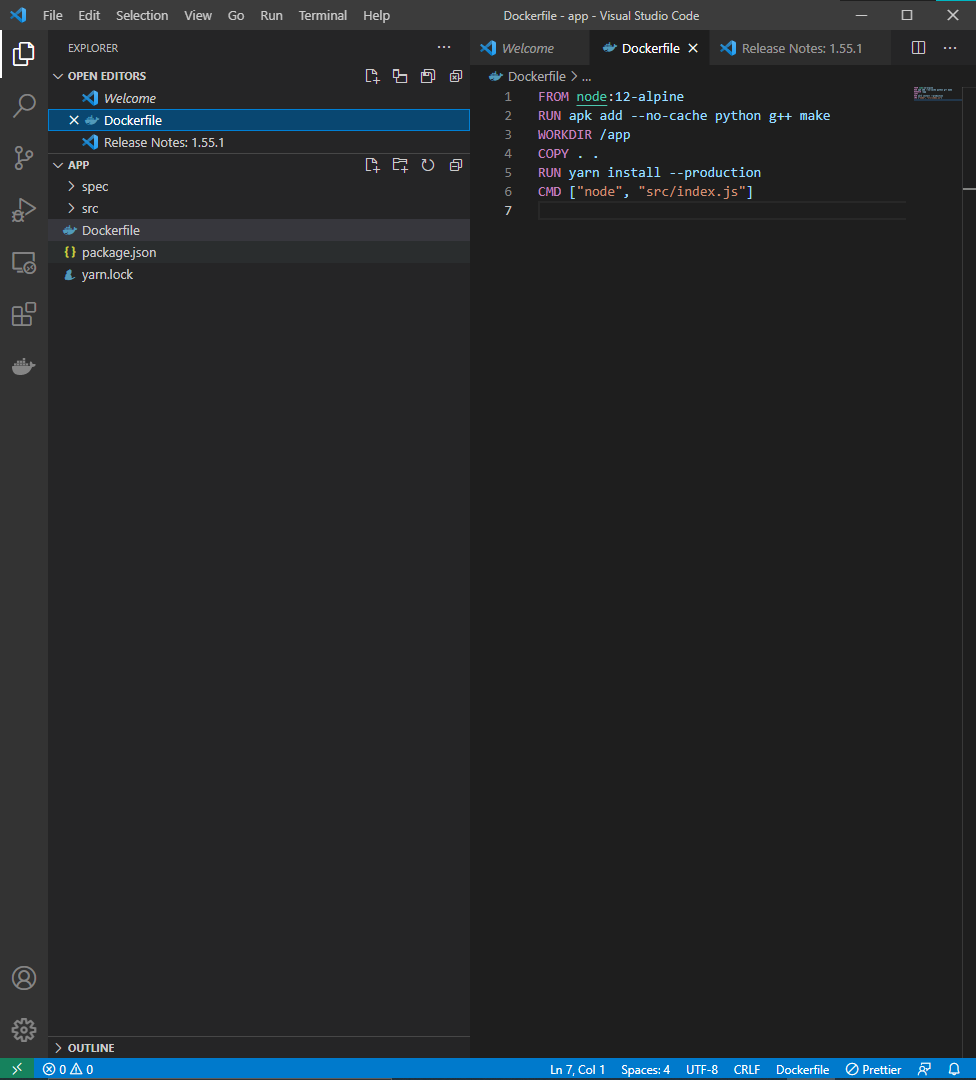
\includegraphics[width=\linewidth]{img/dockerSample.png}
    \label{fig:dockerfilevscode}
    \caption[Een dockerfile in VS code]{de dockerfile om een container  te creëren op basis van een node app, getoond in Visual Studio code}
    \centering
\end{figure}


Om ook compose en het verbinden van containers te demonstreren werd de data die demonstratie applicatie gebruikt ook een s weggeschreven naar een MySQL databank die in een eigen container draait. Eerst werd dit gedaan door een door Docker aangeboden container te gebruiken om zo een verkenning te doen van het netwerk waarop je Docker instantie staat. Met deze verkenner is het mogelijk om de juiste verbinding tussen de demo app en een mysql databank te leggen. Omdat het manueel verbinden moeilijk kan zijn werd ook Docker compose uitgelegd. Met een YAML-file kan je nodige containers definiëren en confituren dat bij het oproepen van composer ze samen opgestart worden en onmiddellijk verbonden zijn. Deze gebundelde containers worden ook samen getoond in de interface van de desktop applicatie.


\paragraph{Ervaring}
Docker’s gebruik is eenvoudig en is ook veel over te vinden online bij eventuele problemen.  De dokker desktop geeft een grafische interface voor het beheren van draaiende containers en images, maar dit is ook allemaal mogelijk via CLI. Met de voorwaarde hier dat bij het overnemen van commando’s deze soms over meerdere regels gespreid zijn en dus dat de commando prompt van Windows niet voldoende is en overgeschakeld moet worden naar powershell.  De desktop interface maakt het wel gemakkelijk om te beheren of dat je lokale Docker instantie draait waardoor het perfect mogelijk is om het geïnstalleerd te hebben staan en buiten gebruik niet door beïnvloed worden. Het starten en stoppen van Docker in een Linux omgeving is te doen via het proces beheer van Linux zelf.  De configuratie bestanden voor containers zijn geschreven in YAML en Visual studio code heeft zelf extensie om specifiek de Docker bestanden te ondersteunen.

\subsection{Fedora Podman}
Dit werd uitgevoerd in een VM met 4 GB ram en 20 gb harde schijfruimte
\paragraph{Installatie en set-up}
Bij de verse installatie van een Fedora workstation versie 53 was Podman al inbegrepen en was er geen nood om hem te installeren.

\paragraph{Ingebruikname}
Het reproduceren van de stappen van de Docker tutorial lukte eerst goed.  Het pullen, builden of draaien van images lukt analoog als met de Docker engine. Inclusief het gebruiken van dezelfde bestanden voor het definiëren van een container vooraleer deze te builden. Figuur \ref{fig:podmanbuild} toont het aanmaken van de container images met podman en figuur \ref{fig:podmanrun} toont hoe het effectief opgestart is.  Bij het persisteren met volumes is ook geen verschil.
\begin{figure}[h]
    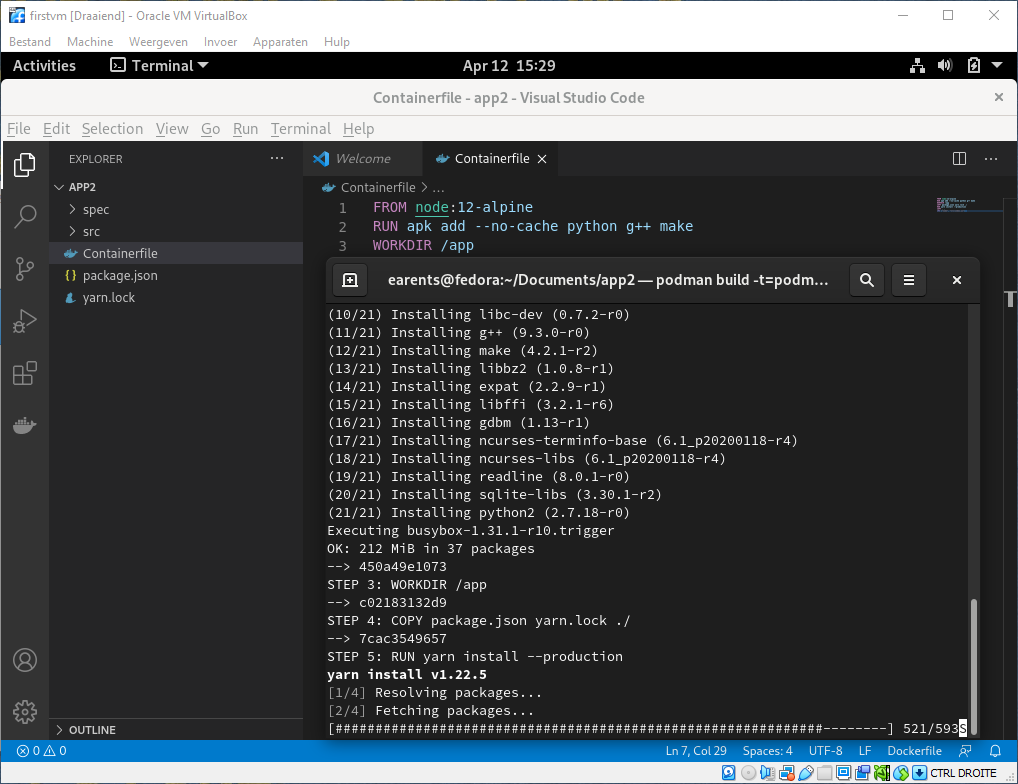
\includegraphics[width=\linewidth]{img/podmanbuild.png}
    \label{fig:podmanbuild}
    \caption[Een dockerfile in VS code om met podman te builden]{Hier maakt Podman met het inhoudelijk zelfde docker-/containerfile as Docker een image}
    \centering
\end{figure}
\begin{figure}[h]
    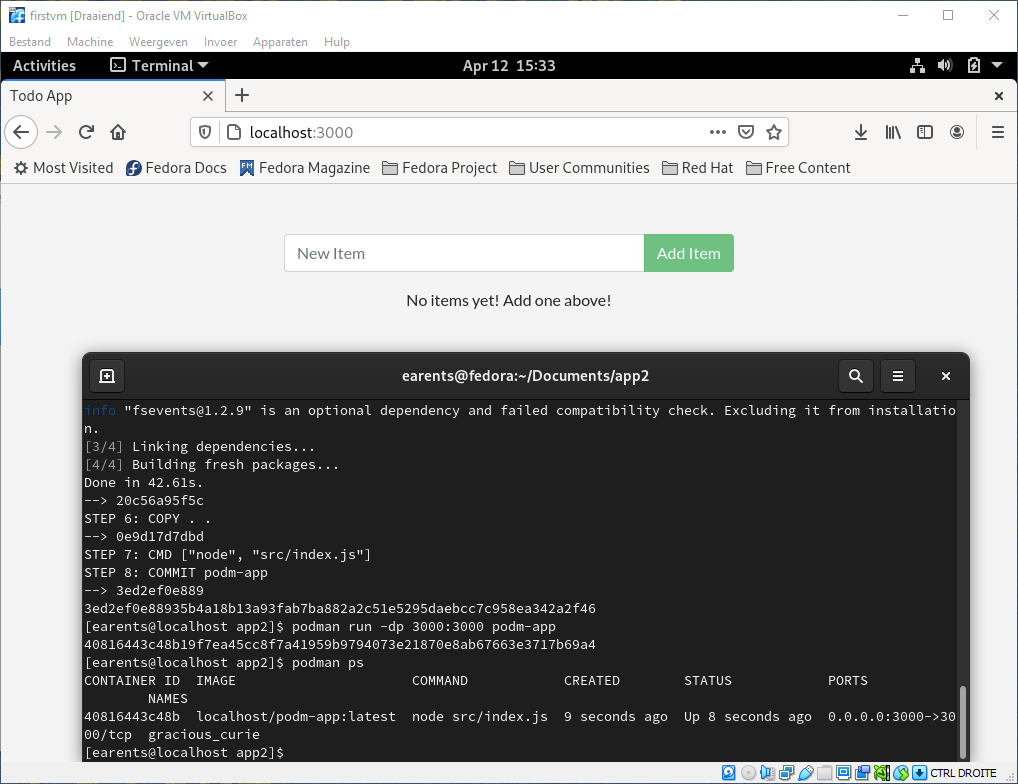
\includegraphics[width=\linewidth]{img/podmanrun.png}
    \label{fig:podmanrun}
    \caption[Podman die een web ap uitvoert]{hier is via command line de aangemaakte container gestart en wort deze op de achtergrond getoont in een webbrowser}
    \centering
\end{figure}

Bij Podman was het lokaal verbinden moeilijker. Het werken met Podman ingebouwde pods is minder goed uitgelegd dan het werken met Docker en het manueel verbinden.  Er bestaat ook een project om Docker compose na te bootsen voor Podman genaamd Podman Compose\footnote{\url{https://GitHub.com/containers/Podman-compose}} .  Hiermee kan je ook onmiddellijk meerdere containers samen laten bundelen en draaien, echter ook hier is het werken met de pod om de juiste poorten te zetten om te kunnen zien of dat het werkt een probleem.

\paragraph{Ervaring}
Het werken met Docker en Podman voor eenvoudige containers te draaien lijkt sterk op elkaar, veel commando’s zijn hetzelfde en geven ook een gelijkaardig resultaat. Doordat het standaard met Fedora gebundeld is was de installatie geen probleem. Ook moet voor het te kunnen gebruiker niet zelf de lokale Podman runtime starten vooraleer je deze kan gebruiken. Echter het werken met de pods van Podman is moeilijker dan met de eenvoudige verbinding die je met Docker kan leggen.

\subsection{Ubuntu Podman}
Dit werd uitgevoerd op een VM met 4gb ram en 30 GB geheugen ruimte. Initieel was die intentie om ook hier Podman een op uit te oefenen.

\paragraph{Installatie en set-up}
Na een basis installatie van Ubuntu LTS 20.4 is er initieel geprobeerd om een installatie te doen van Podman. Volgens de help pagina’s van Podman is het mogelijk op Podman te draaien op Ubuntu. Bij het instaleren op de manieren uitgelegd is er nooit succesvol een installatie gebeurt. Na een tijd tevergeefs te zoeken naar oorzaken is er overschakelt naar het uitproberen van een ander alternatief, namelijk Containerd.
Door lokaal Golang te hebben moet het mogelijk zijn om via Containerd te werken voor container runtime. Ook hier voor het effectief installeren van Golang ondervond ik problemen.  Eens Golang geïnstalleerd lukte het echter niet om Containerd uit te voeren.

\paragraph{Ervaring}
Het is dus niet gelukt om zowel Podman als Containerd uit te voeren op Ubuntu. Voor het installeren van Podman kan het probleem zijn dat ten tijde van het proberen de repositories die Ubuntu aanreikte niet voorzien van de nodige bestanden. Voor Containerd zal het probleem liggen tussen gelijkaardige installatie problemen voor Golang. Dit gekoppeld met dat ik geen ervaring heb met Go heeft ervoor gezorgd dat ook Containerd niet lukte om uit te voeren.

\subsection{Kubernetes gebundeld met Docker desktop}
Dit werd opnieuw uitgevoerd aan de hand van de desktop installatie direct op de laptop. Voor de effectieve uitvoering van Kubernetes werd er gekeken naar het gebruik van GitHub als repository voor images.
\paragraph{Installatie en set-up}
Een volwaardige instantie van Kubernetes is gebundeld met de Docker desktop applicatie. Dit betekent wel dat het op Linux systemen niet gelijkaardig zal zijn.
Voor de GitHub Container Registry is het ten tijde van dit onderzoek nodig om manueel deel te nemen aan de beta versie. Ook stelt GitHub voor om een access token te maken voor het inloggen en verbinden met je container registry.

\paragraph{Ingebruikname}
Het weken met de GitHub container registry lukte vlot. Er zijn twee stappen die je moet doen vooraleer je kan pushen naar je registry. Met je access token kan je via de command line van Docker inloggen op het domein van de GitHub container registry Ghcr.io. Om dan effectief te pushen moet je nog wat aanpassen om lokaal duidelijk te maken dat je naar Ghr.io, om dit te doen moet de lokale container getagd worden en verwijzen naar de ghcr.io/username/containername vooraleer je deze kan pushen. Deze expliciete verwijzing is nodig want Docker zal standaard altijd de Docker hub gebruiken al remote locatie. Het pullen van images van de container registry gebeurt door manueel te specifiëren dat er van daar moet worden gepulled om zo het niet op Dockers hub te zoeken.

De gebundelde Kubernetes van de Docker desktop lukte niet om te gebruiken. Bij het opstarten van Kubernetes via de desktop worden alle nodige onderdelen geïmporteerd en opgestart in hun eigen containers. Kubernetes is niet volledig kunnen starten. Windows task manager gaf aan dat de laptops processor en ram geheugen overbelast werden. Verder toonde de interface van Docker desktop hoe bepaalde containers voor de werking opstartte, afgebroken werden en weer opgestart werden.

\paragraph{Ervaring}
Het werken met de GitHub Container Registry loopt vlot het voornaamste jammerlijke is dat zelfs als je inlogt op de registry dat Docker altijd nog eerst zal proberen met de Docker hub.
Zoals aangegeven lukte Kubernetes niet. Dit zal voornamelijk liggen aan de verouderde laptop die gebruikt werd, gecombineerd met dat de Kubernetes instantie veel eist. De laptop voldoet aan de minimumvereisten volgen de Docker help pagina’s maar mogelijk zijn niet van toepassing op de inbegrepen Kubernetes.  


\subsection{Podman met Minikube voor Kubernetes}
In een Fedora workstation 53 VM met 4 GB ram, twee virtuele CPU’s en 32 GB harde schijfruimte Ook werd er eerst geoefend om te zien of Podman met de GitHub Container Registry kan werken.
\paragraph{Installatie en set-up}
Voor de VM kwam er wat extra set up bij wan Minikube vraagt voor minstens 20 gigabyte vrij en 2 processoren.
Minikube raad ook aan om Cri-o te hebben om Podman te gebruiken als engine in plaats van Docker. Dus dit werd ook geïnstalleerd, op basis van cri-o help pagina’s.  Ook werd Minikube zelf geïnstalleerd.

\paragraph{Ingebruikname}
Het werken met de GitHub container registry in Podman is volledig analoog met de werking in Docker. Podman zoek ook standaard eerst op Docker hub dus moet er manueel gespecificeerd worden dat je een ander registry wilt gebruiken. Tijdens het werken met Podman en GitHub werd er ook een recent gepubliceerd blog van de Fedora Magazine die eens overloopt hoe je met Podman minder grote container images kan maken. Door in het Dockerfile of container file voor je container image optionele dependencies en feature die standaard in je base image staan te verwijderen kan je image grootte verkleind worden. De blog gaf ook een voorbeeld voor het werken met Buildah voor het maken van een image zonder een base image te hebben, maar installatie van Buildah lukte niet.

De ondersteuning die Minikube heeft voor Podman op het moment van dit onderzoek in nog steeds in een experimentele fase. Bij een eerste keer proberen starten van Minikube met Podman en Cri-o voor driver en effectieve runtime kwam er een gekende fout. Het oplossen van deze fout die eigen is aan Podman wordt uitgelegd op de Minikube help pagina’s voor Podman\footnote{\url{https://minikube.sigs.k8s.io/docs/drivers/Podman/}} . Door de fout op te lossen kan Minikube, en alle emoticons die het gebruikt, gestart worden.

Eens Minikube opgestart kan met een lokale instantie van Kubernetes gewerkt worden. Minikube komt met de command line interface voor Kubernetes. Zo is het mogelijk om aan Minikube doorgegeven welke kubectl commando’s moeten worden uitgevoerd. Het is echter ook mogelijk om individueel kubectl te installeren, Minikube zal bij het opstarten er zelf voor zorgen dat deze lokale installatie uitgevoerd wordt op de cluster die Minikube beheerd.  Minikube commando’s staan in voor het beheren van de cluster in zijn geheel zoals het starten stoppen of blootstellen van containers naar buiten. Kubectl is de tool om te werken binnen de cluster en met de containers erin.
\begin{figure}[h]
    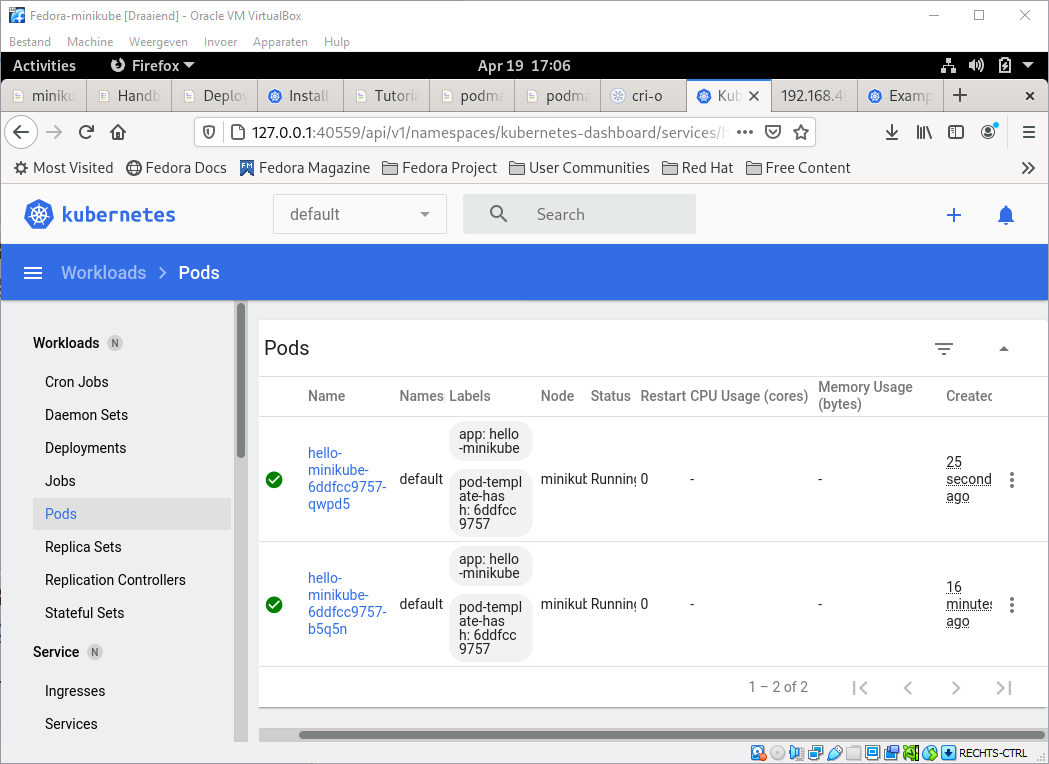
\includegraphics[width=\linewidth]{img/kubenetesDash.png}
    \label{fig:kubenetesDash}
    \caption[the kubenetes Dashboard]{hier toont de Kubernetes dashboard dat een nieuwe pod van de hellominikube container recent gestart is}
    \centering
\end{figure}

Met de lokale Kubernetes instantie is het verder gelukt om Kubernetes uit te proberen. Op basis van een standaardvoorbeeld voor Wordpress en MySQL\footnote{\url{https://kubernetes.io/docs/tutorials/stateful-application/mysql-wordpress-persistent-volume/}}  lukt het om snel de nodige Kustomization.yaml file aan te maken een door te geven aan Kubernetes via kubectl. Het openzetten naar buiten toe gaat dan via Minikube. Verder laat Minikube je ook toe om vlug de browser gebaseerde dashboard, figuur \ref{fig:kubenetesDash}, van je lokale instantie te openen. Hiermee kan je veel van de functionaliteiten van Kubernetes ook doen. Inclusief een publieke image van de GitHub container registry via deze interface pullen en onmiddellijk starten. Kubernetes heeft echter geen voor de hand liggende methode om lokaal bewaarde images of private images te gebruiken bij het starten van een container.

\paragraph{Ervaring}
Podman met GitHub container registry was zeer makkelijk en was zoals vermeld volledig analoog aan de Docker methode. De blogpost gaf een korte uitleg over hoe een container file verder aangepast kan worden om bepaalde zaken te configureren. Jammer genoeg lukte Buildah niet door een conflict tijdens de installatie met de al geïnstalleerde Podman. Buildah zou ook enkel nodig zijn om vanaf nul een nieuwe image te maken en zo zou podman woldoende zijn als er altijd een bestaande image als vertkerlpunt wordt gebruikt.

Het starten van Minikube met Podman vergt wat meer configuratie maar is niet onredelijk. Het gebruikt veel emoticons om berichten te accentueren wat afhankelijk van persoonlijke smaak een minpunt kan zijn. Eens de Minikube Kubernetes gestart is merk je niet meer waarop het effectief draait. Ook is Minikube licht genoeg om zonder problemen te werken met 4 GB ram, iets wat de Docker desktop Kubernetes niet kon.

Kubernetes zelf is zeer goed. Er zijn veel voorbeelden voor te vinden en werkt binnen Minikube. De Dashboard van Kubernetes is ook een zeer grote pluspunt. Het laat een gebruiker toe om de volledige cluster te beheren zonder noodzakelijk via de commandolijn te werken. Ook toont het bij het kiezen van een actie met het dashboard wat de equivalente commando zou zijn om het via command line te doen.


\subsection{Docker engine voor Nomad}
Hiervoor weer de Ubuntu deels om te zien of dat het installeren van Docker zou lukken en omdat deze verder al aan alle eisen voor Nomad voldeed.
\paragraph{Installatie en set-up}
De Docker engine installeren en opstarten lukt zonder problemen. Ook het installeren van Nomad zelf gaf geen complicaties.
\paragraph{Ingebruikname}
Na het installeren van de Docker engine werd er eerst getest of dat alles  werkte zoals het direct op de laptop lukte. Hierbij werden geen problemen ondervonden. Hierna werd een dev omgeving Nomad instantie opgestart om eens mee te werken.
\begin{figure}[h]
    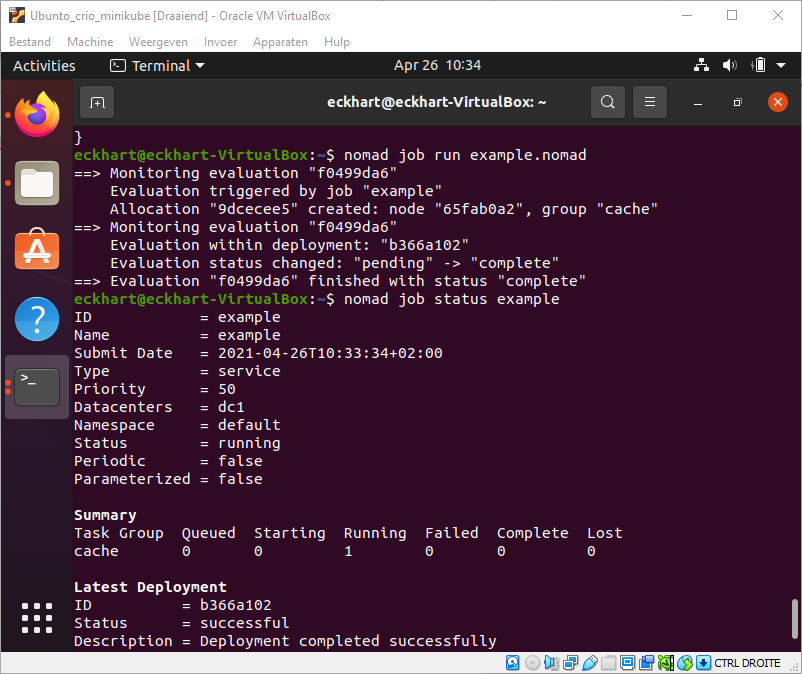
\includegraphics[width=\linewidth]{img/nomadrun.png}
    \label{fig:nomadrun}
    \caption[Een voorbeeld Nomad job]{hier wordt via de cli van Nomad de example.nomad job gestart}
    \centering
\end{figure}
\begin{figure}[h]
    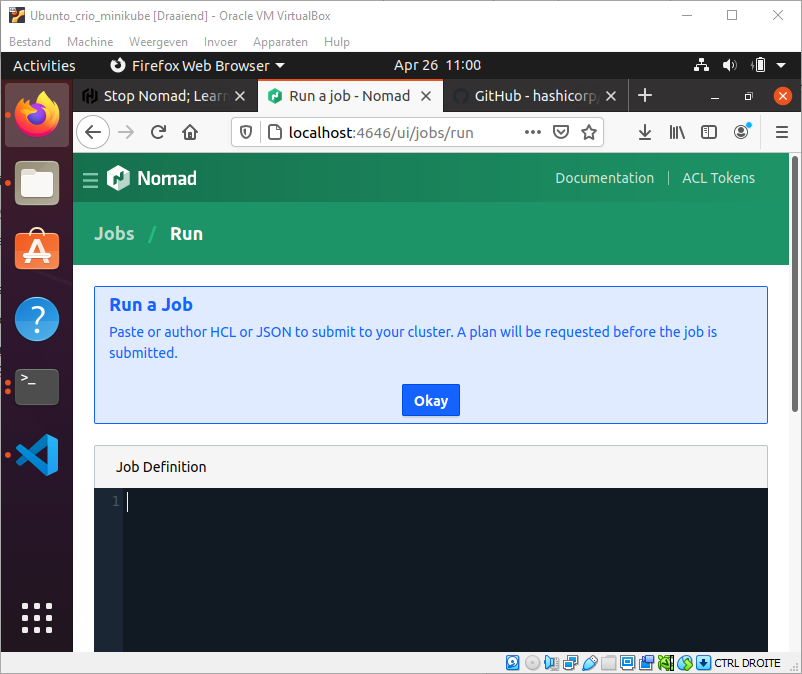
\includegraphics[width=\linewidth]{img/nomdaddash.png}
    \label{fig:nomdaddash}
    \caption[de nomad dashboard]{de dashboard weergave om een job te starten met Nomad}
    \centering
\end{figure}

Hashi Corp heeft een korte tutorial\footnote{\url{https://learn.hashicorp.com/collections/nomad/get-started}} die een inleiding geeft tot het werken met Nomad. Het legt uit wat de workflow is een geeft een voorbeeld toegepast op een kleine container image.  Hier wordt hun eigen .nomad bestandsindeling eens aangehaald die gebruikt wordt voor het configureer van de “jobs” of taken die Nomad moet uitvoeren. Om Nomad iets te laten doen moet eerst een job bestand gemaakt worden. Deze moet vervolgens via command line of de web interface ingepland worden en vervolgens nog eens afzonderlijk uitgevoerd worden. Figuur \ref{fig:nomadrun} toont het starten van een job aan de hand van de cli en figuur \ref{fig:nomdaddash} toont hoe de dashoard een job kan inplannen. Een enkele container draaien en dupliceren lukte maar het achterhalen hoe een Wordpress site te draaien lukte niet.

\paragraph{Ervaring}
Door Nomad werking met jobs voor alle taken is er een duidelijk verschil met Kubernetes. Een groot voordeel is dat Nomad meer kan beheren dan enkel containers. Maar het heeft zeker zijn minpunten. Zo is de eigen markup voor de configuratie een bijkomende barrière voor het werken met Nomad in vergelijking met de al veelgebruikte YAML die Docker, Podman en Kubernetes allemaal gebruiken.  Visual studio code heeft gelukkig een extensie voor de Configuratie Taal die hashicorp gebruikt die het werken met deze .Nomad  bestanden helpt. Nomad heeft ook een web browser gebaseerde interface maar deze toont niet wat een equivalent commando voor de command line zou zijn. Het is ook in het algemeen minder gebruikt dan Kubernetes waardoor uitleg en integratie minder is.  

\section{Samengevatte resultaten software Tests}
%% TODO: insert table comarisons?
Dit deel vergelijkt samengevat eens de technologieën die gebruikt zijn. Enkel voor orchestration is er een duidelijke voorkeur voor Kubernetes als leermiddel.

\subsection{Runtimes}

In basis gebruik lijken Docker en Podman goed op elkaar. De grootste verschillen zitten in de installatie en de eigen werking voor meerdere samenhangende containers. Qua installatie komt Podman standaard geïnstalleerd in Fedora, en moet Docker altijd geïnstalleerd worden. De Docker compose die afhankelijk afzonderlijk geïnstalleerd moet worden maakt het verbinden van container mogelijk  Het equivalent in Podman met de pods is iets complexer en zelfs met een extra overbrugging van Podman Compose niet voor de hand liggend. Echter deze verbinding tussen container kan ook gedaan worden in Kubernetes en is bij gebruik van Kubernetes niet meer zo belangrijk.

Verder is de Docker desktop voor het leren maar een kleine meerwaarde. Het is ten eerste niet beschikbaar op linux systemen. Ten tweede moeten veel functionaliteiten nog via de command line uitgevoerd worden. De desktop applicatie een overzicht van lokale images het maken van een nieuwe image moet via command line interface. Ten derde is de gebundelde Kubernetes zwaarder dan een Kubernetes instantie met Minikube.

\subsection{Repositories}

Tussen de twee gebruikte repository is er niet meteen een de beter is dan de andere. De Docker hub wordt door zowel Docker als Podman gebruikt als standaard doel om image te pushen. Dit beteken dat er weinig aangepast moet worden om effectief te pushen of pullen. Echter de Docker hub zet standaard images publiek en heeft maar een private image mogelijkheid voor gratis accounts. De GitHub container registry daarentegen zou een beetje extra werk vragen om het doel voor het pushen van een image te selecteren. Het zou wel geen extra account nodigen hebben als de student al reeds met GitHub werkt. Over de specifieke kosten en regeling van de GitHub container registry kan er nog geen uitspraak gedaan worden doordat deze nog in bèta fase is. Zou het zelfde limiet  van 500 mb voor private containers gelden als op de rest van GitHub packages zou deze te klein zijn om meer te beteken dan één of enkele private images.

\subsection{Orchestration}

Voor orchestration is Kubernetes de beste van de twee geteste voor het werken met containers. Zo heeft het een dashboard weergave die niet alleen de noodzaak voor het werken via command line minimaliseert, het toont ook bij het uitvoeren van taken via deze dasboard de equivalente commando’s om het via cli te doen. Om met Kubernetes te leren werken is de beschikbaarheid Minikube ook een pluspunt. Minikube helpt om een lokale Kubernetes cluster op te starten en beheren. Verder kan Minikube ook de juiste verbindingen maken om een keuze aan achterliggende runtime te hebben.  Minikube heeft de beste ondersteuning voor Docker als engine maar kan met wat extra configuratie een het installeren kan Cri-o als hulpstuk ook met Podman als runtime werken. één van de grotere minpunten die eigen is aan Kubernetes is dat het moeilijk is om containers te draaien op basis van lokaal bewaarde images of privé bewaard in een repository.

Om specifiek met containers te werken is Nomad minder aan te raden. De hasicorp configuration language is ook een extra stap in het leerproces. Het kan dat een student Yaml dei Kubernetes gebruikt nog niet gezien heeft, maar de kans is groter dat de student ook Yaml elders zal tegenkomen dan de Hasicorp markup. Ook iets dat het leren ten nadele zou komen ten opzichte van Kubernetes is dat de dashboard niet de equivalente commando’s toont, dit is deels toe te kennen aan de methodologie van Nomad om aanpassingen aan je draaiende containers te doen op basis van jobs, die telkens geschreven moeten worden in de hasicorp configuration language.


% Voeg hier je eigen hoofdstukken toe die de ``corpus'' van je bachelorproef
% vormen. De structuur en titels hangen af van je eigen onderzoek. Je kan bv.
% elke fase in je onderzoek in een apart hoofdstuk bespreken.

%\input{...}
%\input{...}
%...

%%=============================================================================
%% Conclusie
%%=============================================================================

\chapter{Conclusie}
\label{ch:conclusie}

% TODO: Trek een duidelijke conclusie, in de vorm van een antwoord op de
% onderzoeksvra(a)g(en). Wat was jouw bijdrage aan het onderzoeksdomein en
% hoe biedt dit meerwaarde aan het vakgebied/doelgroep? 
% Reflecteer kritisch over het resultaat. In Engelse teksten wordt deze sectie
% ``Discussion'' genoemd. Had je deze uitkomst verwacht? Zijn er zaken die nog
% niet duidelijk zijn?
% Heeft het onderzoek geleid tot nieuwe vragen die uitnodigen tot verder 
%onderzoek?

Zeer grof een klad 

best om vm te werken; vereisten min 4gb ram; 2cpu;  meer dan 20 gb schijfruimte, webbrowser en internet.
directe werken met containers is in Fedora met Podman het snelst, voor docker extra installatie en mogelijk zelf daemon regelen. Multicontainer zonder kubernetes is Dockers met compose het zekerst. De rest van runtime zijn te complex, niche of os specifiek.
voor regesteries is Dockers hub het  zekerst, maar kan GitHub beter zijn afhankelijk van de status na de bèta
Kubernetes met Minikube het beste, Nomad niet aan te raden. Andere zijn te specifiek voor os of onmiddellijk Cloud gebaseerd(opensift)
Cloud services, voor maken nieuwe image toch eerst lokaal, dus de rest kan ook lokaal
voor een stappenplan om alles eens te doen. Een image pullen en draaien, op basis van een node of ander applicatie die wegschrijft naar bestanden een image maken. Volume gebruiken voor deze weggeschreven warden te persisteren. Deze eens pushen. In Kubernetes deze zelfde applicatie pullen en draaien, met Kubernetes ook een wordpress instantie starten.




%%=============================================================================
%% Bijlagen
%%=============================================================================

\appendix
\renewcommand{\chaptername}{Appendix}

%%---------- Onderzoeksvoorstel -----------------------------------------------

\chapter{Onderzoeksvoorstel}

Het onderwerp van deze bachelorproef is gebaseerd op een onderzoeksvoorstel dat vooraf werd beoordeeld door de promotor. Dat voorstel is opgenomen in deze bijlage.

% Verwijzing naar het bestand met de inhoud van het onderzoeksvoorstel
%---------- Inleiding ---------------------------------------------------------

\section{Introductie} % The \section*{} command stops section numbering
\label{sec:introductie}

Hier introduceer je werk. Je hoeft hier nog niet te technisch te gaan.

Je beschrijft zeker:

\begin{itemize}
  \item de probleemstelling en context
  \item de motivatie en relevantie voor het onderzoek
  \item de doelstelling en onderzoeksvraag/-vragen
\end{itemize}

%---------- Stand van zaken ---------------------------------------------------

\section{State-of-the-art}
\label{sec:state-of-the-art}

Hier beschrijf je de \emph{state-of-the-art} rondom je gekozen onderzoeksdomein. Dit kan bijvoorbeeld een literatuurstudie zijn. Je mag de titel van deze sectie ook aanpassen (literatuurstudie, stand van zaken, enz.). Zijn er al gelijkaardige onderzoeken gevoerd? Wat concluderen ze? Wat is het verschil met jouw onderzoek? Wat is de relevantie met jouw onderzoek?

Verwijs bij elke introductie van een term of bewering over het domein naar de vakliteratuur, bijvoorbeeld~\autocite{Doll1954}! Denk zeker goed na welke werken je refereert en waarom.

% Voor literatuurverwijzingen zijn er twee belangrijke commando's:
% \autocite{KEY} => (Auteur, jaartal) Gebruik dit als de naam van de auteur
%   geen onderdeel is van de zin.
% \textcite{KEY} => Auteur (jaartal)  Gebruik dit als de auteursnaam wel een
%   functie heeft in de zin (bv. ``Uit onderzoek door Doll & Hill (1954) bleek
%   ...'')

Je mag gerust gebruik maken van subsecties in dit onderdeel.

%---------- Methodologie ------------------------------------------------------
\section{Methodologie}
\label{sec:methodologie}

Hier beschrijf je hoe je van plan bent het onderzoek te voeren. Welke onderzoekstechniek ga je toepassen om elk van je onderzoeksvragen te beantwoorden? Gebruik je hiervoor experimenten, vragenlijsten, simulaties? Je beschrijft ook al welke tools je denkt hiervoor te gebruiken of te ontwikkelen.

%---------- Verwachte resultaten ----------------------------------------------
\section{Verwachte resultaten}
\label{sec:verwachte_resultaten}

Hier beschrijf je welke resultaten je verwacht. Als je metingen en simulaties uitvoert, kan je hier al mock-ups maken van de grafieken samen met de verwachte conclusies. Benoem zeker al je assen en de stukken van de grafiek die je gaat gebruiken. Dit zorgt ervoor dat je concreet weet hoe je je data gaat moeten structureren.

%---------- Verwachte conclusies ----------------------------------------------
\section{Verwachte conclusies}
\label{sec:verwachte_conclusies}

Hier beschrijf je wat je verwacht uit je onderzoek, met de motivatie waarom. Het is \textbf{niet} erg indien uit je onderzoek andere resultaten en conclusies vloeien dan dat je hier beschrijft: het is dan juist interessant om te onderzoeken waarom jouw hypothesen niet overeenkomen met de resultaten.



%%---------- Andere bijlagen --------------------------------------------------
\chapter{Configuratie bestanden}
Wegens de omvang van deze configuratie bestanden zijn deze hier toegevoegd.

\section{mysql-deployment.yaml}\label{K8sql}
\lstinputlisting{configs/mysql-deployment.yaml}
\section{wordpress-deployment.yaml}\label{K8wp}
\lstinputlisting{configs/wordpress-deployment.yaml}
\lstset{%
    breaklines=true,
    breakatwhitespace=true,
}%%zondr dit is het comentaar in het job bestan te lang om op een pagina te staan
\section{example.nomad}\label{nomadjobconfig}
\lstinputlisting{configs/example.nomad}[]
%\input{...}

%%---------- Referentielijst --------------------------------------------------

\printbibliography[heading=bibintoc]

\end{document}
